% n^2+n+41: small prime values, Euler's fortieth index, then 41^2.
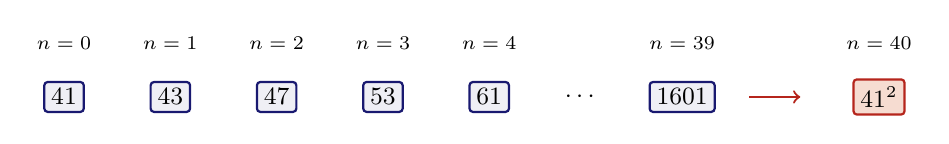
\begin{tikzpicture}[x=1cm,y=1cm]
  \foreach \x/\n/\v in {0/0/41, 1.35/1/43, 2.7/2/47, 4.05/3/53, 5.4/4/61} {
    \node[font=\scriptsize,anchor=south] at (\x,0.48) {$n=\n$};
    \node[draw=MidnightBlue,thick,rounded corners=1.2pt,fill=MidnightBlue!7,
          inner sep=2.5pt,font=\small] at (\x,0) {$\v$};
  }
  \node[font=\small] at (6.55,0) {$\cdots$};
  \node[font=\scriptsize,anchor=south] at (7.85,0.48) {$n=39$};
  \node[draw=MidnightBlue,thick,rounded corners=1.2pt,fill=MidnightBlue!7,
        inner sep=2.5pt,font=\small] at (7.85,0) {$1601$};
  \draw[BrickRed,thick,->] (8.7,0) -- (9.35,0);
  \node[font=\scriptsize,anchor=south] at (10.35,0.48) {$n=40$};
  \node[draw=BrickRed,thick,rounded corners=1.2pt,fill=BrickRed!12,
        inner sep=2.5pt,font=\small] at (10.35,0) {$41^{2}$};
\end{tikzpicture}
